
\documentclass[14pt]{beamer}

\usepackage{color}
\usepackage{tikz}
\usepackage{graphicx}

\usetheme{Warsaw}

\newcommand{\CC}{C\nolinebreak\hspace{-.05em}\raisebox{.4ex}{\tiny\bf +}\nolinebreak\hspace{-.10em}\raisebox{.4ex}{\tiny\bf +}}

\begin{document}

  {
  \usebackgroundtemplate{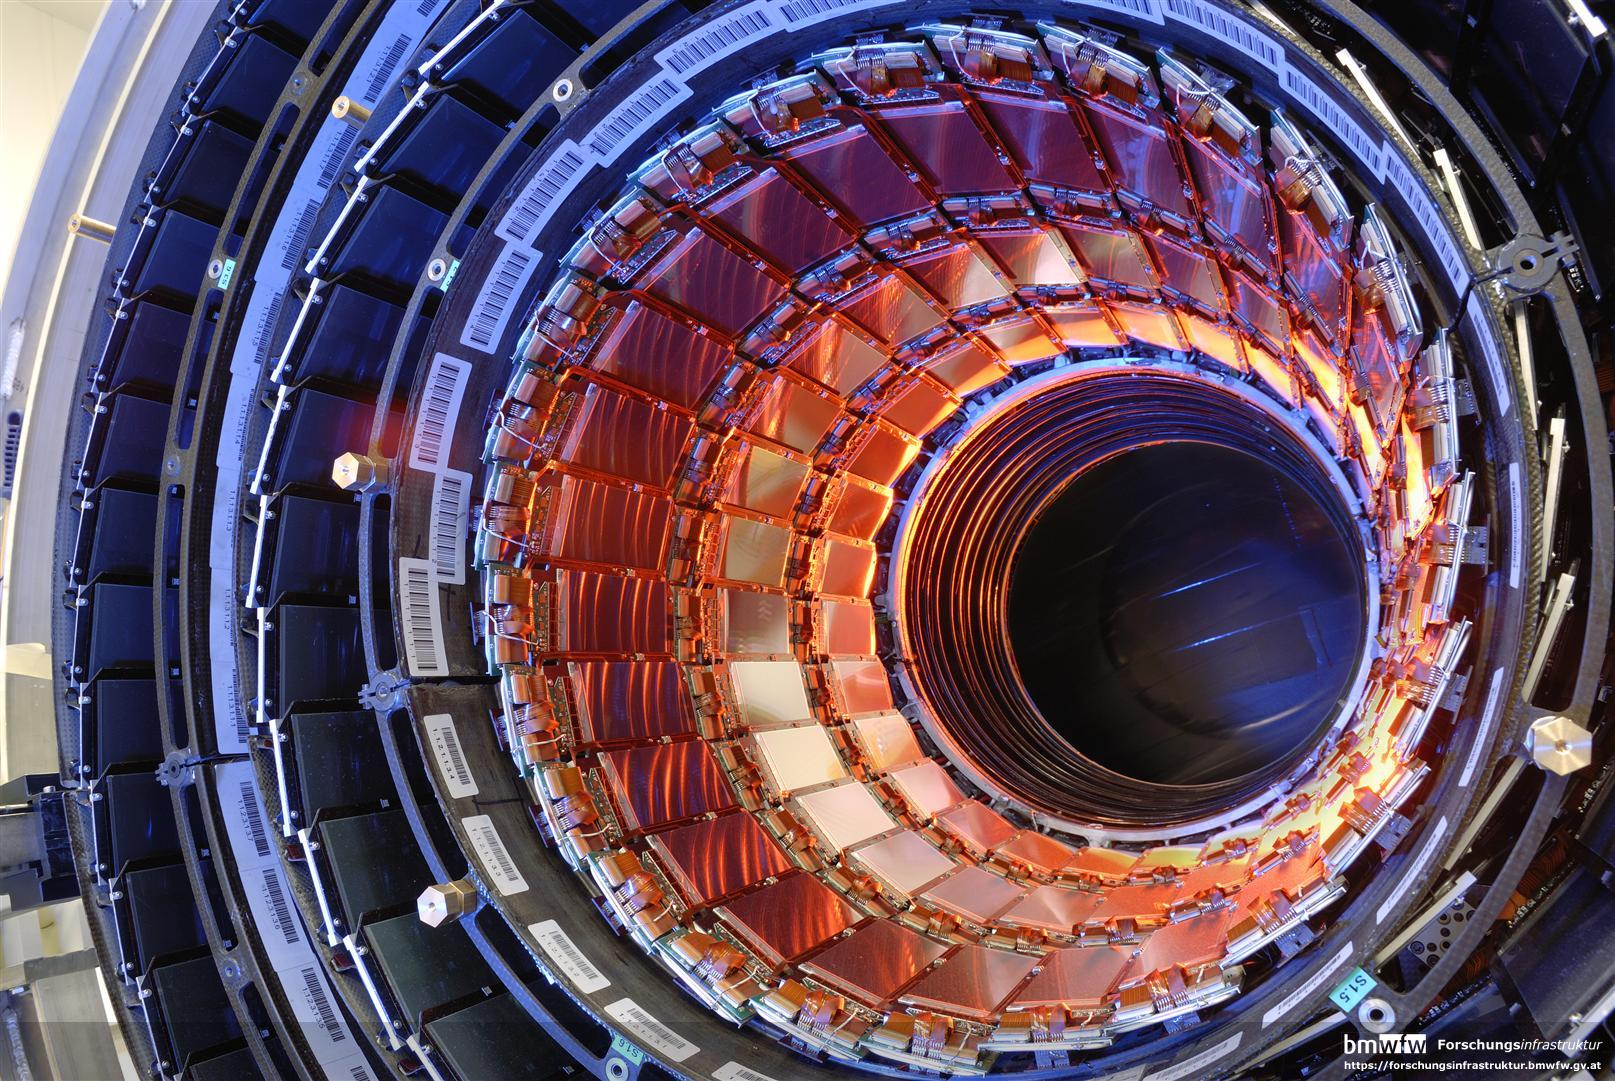
\includegraphics[width=\paperwidth, height=\paperheight]{images/cms.jpg}}
\begin{frame}

\setbeamercolor{author}{fg=white}
\setbeamercolor{date}{fg=white}
\title{Simulation of a particle detector}
\author{Arnaud Schils \\ Simon Lardinois}
\maketitle

\end{frame}
}

\begin{frame}
\frametitle{Summary}

\begin{enumerate}
  \setlength\itemsep{1.4em}
  \item Problem statement
  \item The software \textit{pdetect}
  \begin{itemize}
    \item Geometries and boundary conditions
    \item Computing the \textcolor{red}{potential} in the detector
    \item Computing the \textcolor{red}{current} induced by a particle
  \end{itemize}
  \item Conclusion
\end{enumerate}
\end{frame}

\begin{frame}

\frametitle{Problem statement}
\framesubtitle{The detector}

%\textcolor{red}{strips}: cathode

\begin{figure}[H]
\begin{center}
	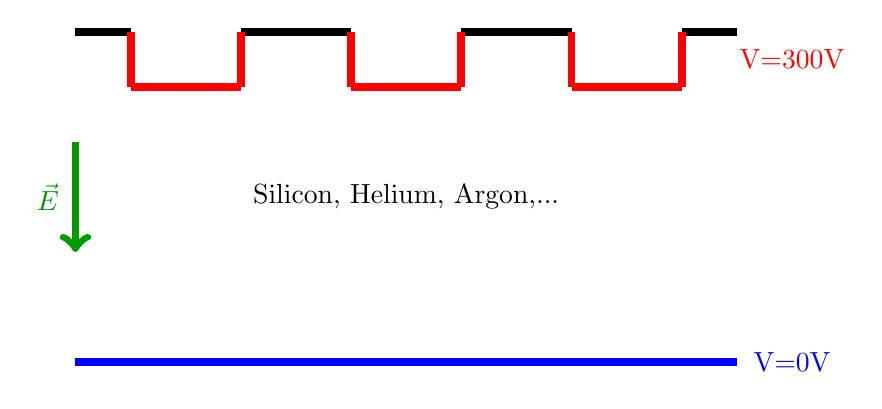
\begin{tikzpicture}[scale=0.7]
    \draw[line width=1mm, black] (-6,3) -- (-5,3);
    \draw[line width=1mm, black] (-3,3) -- (-1,3);
    \draw[line width=1mm, black] (1,3) -- (3,3);
    \draw[line width=1mm, black] (5,3) -- (6,3);

    \draw[line width=1mm, red] (-5,2) -- (-3,2);
    \draw[line width=1mm, red] (-1,2) -- (1,2);
    \draw[line width=1mm, red] (3,2) -- (5,2);

    \draw[line width=1mm, red] (-5,3) -- (-5,2);
    \draw[line width=1mm, red] (-3,3) -- (-3,2);

    \draw[line width=1mm, red] (-1,3) -- (-1,2);
    \draw[line width=1mm, red] (1,3) -- (1,2);

    \draw[line width=1mm, red] (3,3) -- (3,2);
    \draw[line width=1mm, red] (5,3) -- (5,2);

    \draw[line width=1mm, blue] (-6,-3) -- (6,-3);
    \node[blue] at (7,-3) {V=0V};
    \node[red] at (7,2.5) {V=300V};
    \node at (0,0) {Silicon, Helium, Argon,...};

    \node[black!40!green] at (-6.5,0) {$\vec{\text{E}}$};
    \draw[line width=1mm, black!40!green, ->] (-6, 1) -- (-6,-1);


	\end{tikzpicture}
\end{center}
\end{figure}

\end{frame}

\begin{frame}
  \frametitle{Problem statement}
  \framesubtitle{Media ionization}


  \begin{figure}[H]
  \begin{center}
  	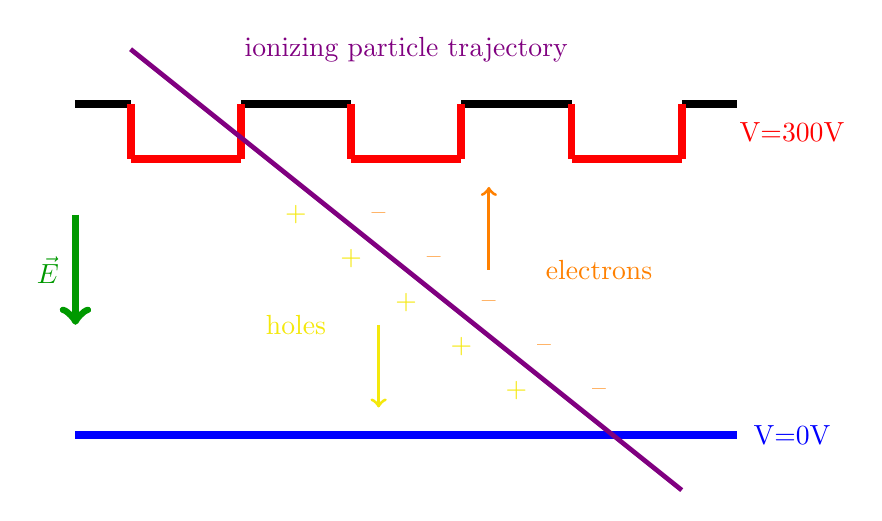
\begin{tikzpicture}[scale=0.7]
      \draw[line width=1mm, black] (-6,3) -- (-5,3);
      \draw[line width=1mm, black] (-3,3) -- (-1,3);
      \draw[line width=1mm, black] (1,3) -- (3,3);
      \draw[line width=1mm, black] (5,3) -- (6,3);

      \draw[line width=1mm, red] (-5,2) -- (-3,2);
      \draw[line width=1mm, red] (-1,2) -- (1,2);
      \draw[line width=1mm, red] (3,2) -- (5,2);

      \draw[line width=1mm, red] (-5,3) -- (-5,2);
      \draw[line width=1mm, red] (-3,3) -- (-3,2);

      \draw[line width=1mm, red] (-1,3) -- (-1,2);
      \draw[line width=1mm, red] (1,3) -- (1,2);

      \draw[line width=1mm, red] (3,3) -- (3,2);
      \draw[line width=1mm, red] (5,3) -- (5,2);

      \draw[line width=1mm, blue] (-6,-3) -- (6,-3);
      \node[blue] at (7,-3) {V=0V};
      \node[red] at (7,2.5) {V=300V};

      \node[black!40!green] at (-6.5,0) {$\vec{\text{E}}$};
      \draw[line width=1mm, black!40!green, ->] (-6, 1) -- (-6,-1);

      \draw[line width=0.6mm, violet] (-5, 4) -- (5, -4);
      \node[violet] at (0,4) {ionizing particle trajectory};
      \node[black!5!yellow] at (-2,1) {+};
      \node[black!5!yellow] at (-1,0.2) {+};
      \node[black!5!yellow] at (0,-0.6) {+};
      \node[black!5!yellow] at (1,-1.4) {+};
      \node[black!5!yellow] at (2,-2.2) {+};

      \node[black!5!yellow] at (-2,-1) {holes};
      \draw[line width=0.4mm, black!5!yellow, ->] (-0.5,-1) -- (-0.5,-2.5);

      \node[orange] at (-0.5,1) {--};
      \node[orange] at (0.5,0.2) {--};
      \node[orange] at (1.5,-0.6) {--};
      \node[orange] at (2.5,-1.4) {--};
      \node[orange] at (3.5,-2.2) {--};

      \node[orange] at (3.5,0) {electrons};
      \draw[line width=0.4mm, orange, ->] (1.5,0) -- (1.5,1.5);

  	\end{tikzpicture}
  \end{center}
  \end{figure}

\end{frame}

\begin{frame}
  \frametitle{Problem statement}
  \framesubtitle{Drift velocity}

  Charges drift with \textcolor{red}{velocity}

  \[|\vec{v}| = \mu |\vec{E}|\]

  where  $\mu$ is the \textcolor{red}{mobility}

  \begin{itemize}
    \item \textcolor{red}{Electrons mobility} is much \textcolor{red}{higher} than hole mobility
    \item mobility decreases when fields of 104 $V cm^{-1}$ and higher are
    applied due to \textcolor{red}{saturation}

  \end{itemize}
\end{frame}

\begin{frame}
  \frametitle{Problem statement}
  \framesubtitle{Shockley Ramo theorem}

   Instantaneous \textcolor{red}{current} generated	by \textcolor{red}{one moving charge} $q$ at speed $\vec{v}$

		\[i_{e,h}(t) = -q \vec{v}(t) \cdot \vec{E}_w(t)\]

	\textcolor{red}{Weighting field} $\vec{E}_w$ = $\vec{E}$ computed when applying

\begin{itemize}
  \item $1V$ to the measurement electrode
	\item $0V$ to the other electrodes
\end{itemize}

\textcolor{red}{Instantaneous current} induced by the particle

\[i_{tot}(t) = \sum_{holes} i_h(t) + \sum_{electrons} i_e(t)\]
\end{frame}

\begin{frame}
  \frametitle{Problem statement}
  \framesubtitle{Townsend avalanche}

\begin{itemize}
 \item $e^{-}$ extract $e^{-}$ from media molecules
 \item In \textcolor{red}{gas detectors} when $|\vec{E}| > 10^6$Vm$^{-1}$
\end{itemize}

\begin{center}
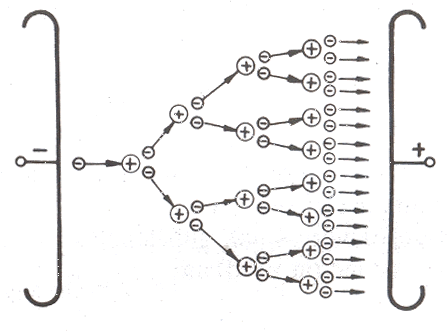
\includegraphics[scale=0.35,angle=90]{images/townsend_avalanche.png}
\end{center}

\end{frame}

\begin{frame}
  \frametitle{Problem statement}
  \framesubtitle{Summary: what do we need to compute the current?}

  \vspace{-2em}


\[i = -q \vec{v} \cdot \vec{E}_w \qquad \qquad \quad \vec{v} = \frac{q}{|q|} \mu \vec{E}\]

\[\implies i = - |q| \mu \textcolor{red}{\vec{E}} \cdot \textcolor{red}{\vec{E}_w}\]

\[\vec{E} = -\nabla V \qquad \qquad \vec{E}_w = -\nabla V_w\]

\vspace{1em}

$\implies$ to compute $i$ you need \textcolor{red}{$V$} and \textcolor{red}{$V_w$}

$\implies$ Solve \textcolor{red}{$\nabla^2 V = 0$} and
\textcolor{red}{$\nabla^2 V_w = 0$} for corresponding boundary conditions

\end{frame}

\begin{frame}
  \frametitle{Pdetect software}
  \framesubtitle{Features}

\begin{itemize}
  \item Simulates both \textcolor{red}{silicon and gas detectors}
  \item Computes \textcolor{red}{$\vec{E}$} and \textcolor{red}{$\vec{E}_w$}
  for \textcolor{red}{three} different 2D \textcolor{red}{geometries}
  \item Computes \textcolor{red}{$i_{tot}$} for any particle trajectory
  \begin{itemize}
  \item Simulates \textcolor{red}{Townsend avalanche} and \textcolor{red}{mobility saturation}
  \end{itemize}
  \item Outputs:
  \begin{itemize}
      \item plots of $V(x,y)$,$V_w(x,y)$, $\vec{E}(x,y)$, $\vec{E}_w(x,y)$
      \item points $(t,i_{tot}(t))$ in a text file
  \end{itemize}
\end{itemize}

\end{frame}

\begin{frame}
  \frametitle{Pdetect software}
  \framesubtitle{Technical characteristics}

  Developed in \textcolor{red}{\CC} (5209 lines of code)
\newline

\textcolor{red}{Object oriented programming} (inheritance, generic programming,
composition,...) advantages:

  %\begin{itemize}
    %\item Model-view-controller (\textcolor{red}{MVC}) design pattern
    %\item Intensive use of \textcolor{red}{OO} (inheritance, generic programming, composition,...)
  %\end{itemize}

\begin{itemize}
  \item \textcolor{red}{avoids code duplication}
  \item \textcolor{red}{add features} to a module with \textcolor{red}{few modifications} to other
  modules
  \item improve code \textcolor{red}{readability}
  \newline
\end{itemize}

\textcolor{red}{Fast}: multithreading, adaptive grid refinement,...

\end{frame}

\begin{frame}
  \frametitle{Pdetect software}
  \framesubtitle{Detector geometry and boundary conditions (I)}

\vspace{-2em}

\begin{figure}[H]
\begin{center}
	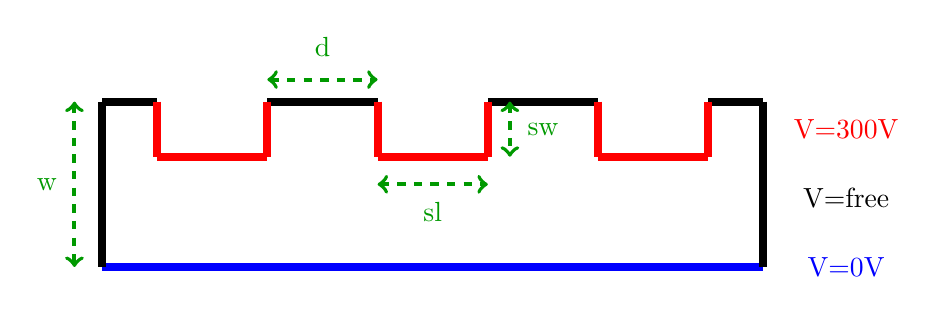
\begin{tikzpicture}[scale=0.7]
    \draw[line width=1mm, black] (-6,3) -- (-5,3);
    \draw[line width=1mm, black] (-3,3) -- (-1,3);
    \draw[line width=0.5mm, black!40!green, <->, dashed] (-3,3.4) -- (-1,3.4);
    \node at (-2, 4) {\textcolor{black!40!green}{d}};

    \draw[line width=1mm, black] (1,3) -- (3,3);
    \draw[line width=1mm, black] (5,3) -- (6,3);

    \draw[line width=1mm, red] (-5,2) -- (-3,2);
    \draw[line width=1mm, red] (-1,2) -- (1,2);
    \draw[line width=0.5mm, black!40!green, <->, dashed] (-1,1.5) -- (1,1.5);
    \node at (0, 1) {\textcolor{black!40!green}{sl}};
    \draw[line width=1mm, red] (3,2) -- (5,2);

    \draw[line width=1mm, red] (-5,3) -- (-5,2);
    \draw[line width=1mm, red] (-3,3) -- (-3,2);

    \draw[line width=1mm, red] (-1,3) -- (-1,2);
    \draw[line width=1mm, red] (1,3) -- (1,2);
    \draw[line width=0.5mm, black!40!green, <->, dashed] (1.4,3) -- (1.4,2);
    \node at (2, 2.5) {\textcolor{black!40!green}{sw}};

    \draw[line width=1mm, red] (3,3) -- (3,2);
    \draw[line width=1mm, red] (5,3) -- (5,2);

    \draw[line width=1mm, blue] (-6,0) -- (6,0);
    \node[blue] at (7.5,0) {V=0V};
    \node at (7.5, 1.25) {V=free};
    \node[red] at (7.5,2.5) {V=300V};

    \draw[line width=1mm, black] (-6,3) -- (-6,0);
    \draw[line width=0.5mm, black!40!green, <->, dashed] (-6.5,3) -- (-6.5,0);
    \node at (-7, 1.5) {\textcolor{black!40!green}{w}};
    \draw[line width=1mm, black] (6,3) -- (6,0);

	\end{tikzpicture}
\end{center}
\end{figure}

\begin{columns}
  \begin{column}{0.5\textwidth}

    \begin{itemize}
      \item number of strips
      \item strip length \textcolor{black!40!green}{sl}
      \item strip width \textcolor{black!40!green}{sw}
    \end{itemize}

  \end{column}

  \begin{column}{0.6\textwidth}
    \begin{itemize}
      \item strip potential \textcolor{red}{V}
      \item detector width \textcolor{black!40!green}{w}
      \item inter-strips distance \textcolor{black!40!green}{d}
    \end{itemize}

  \end{column}
\end{columns}

\end{frame}

\begin{frame}
  \frametitle{Pdetect software}
  \framesubtitle{Detector geometry and boundary conditions (II)}

\vspace{-3em}

\begin{figure}[H]
\begin{center}
	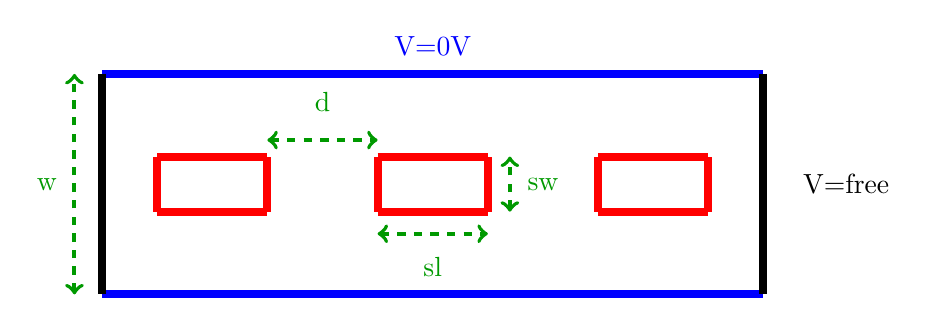
\begin{tikzpicture}[scale=0.7]
    \draw[line width=1mm, blue] (-6,3.5) -- (6,3.5);
    \draw[line width=1mm, blue] (-6,-0.5) -- (6,-0.5);
    \node at (0, 4) {\textcolor{blue}{V=0V}};

    \draw[line width=1mm, black] (-6,3.5) -- (-6,-0.5);
    \draw[line width=1mm, black] (6,3.5) -- (6,-0.5);
    \draw[line width=0.5mm, black!40!green, dashed, <->] (-6.5,-0.5) -- (-6.5,3.5);
    \node at (-7, 1.5) {\textcolor{black!40!green}{w}};
    \node at (7.5, 1.5) {\textcolor{black}{V=free}};

    \foreach \x in {-5,-1,3} {
      \foreach \y in {1,2} {
        \draw[line width=1mm, red] (\x,\y)--(\x+2,\y);
      }
    }

    \draw[line width=0.5mm, black!40!green, <->, dashed] (-1,0.6)--(1,0.6);
    \node at (0, 0) {\textcolor{black!40!green}{sl}};

    \foreach \x in {-5,-1,3} {
        \draw[line width=1mm, red] (\x,1)--(\x,2);
        \draw[line width=1mm, red] (\x+2,1)--(\x+2,2);
    }
    \draw[line width=0.5mm, black!40!green, <->, dashed] (1.4,1)--(1.4,2);
    \node at (2, 1.5) {\textcolor{black!40!green}{sw}};

    \draw[line width=0.5mm, black!40!green, <->, dashed] (-3,2.3)--(-1,2.3);
    \node at (-2, 3) {\textcolor{black!40!green}{d}};


    %\draw[line width=0.5mm, black!40!green, <->] (-3,3.4) -- (-1,3.4);
    %\node at (-2, 4) {\textcolor{black!40!green}{d}};
	\end{tikzpicture}
\end{center}
\end{figure}

\begin{columns}
  \begin{column}{0.5\textwidth}

    \begin{itemize}
      \item number of strips
      \item strip length \textcolor{black!40!green}{sl}
      \item strip width \textcolor{black!40!green}{sw}
    \end{itemize}

  \end{column}

  \begin{column}{0.6\textwidth}
    \begin{itemize}
      \item strip potential \textcolor{red}{V}
      \item detector width \textcolor{black!40!green}{w}
      \item inter-strips distance \textcolor{black!40!green}{d}
    \end{itemize}

  \end{column}
\end{columns}

\end{frame}

\begin{frame}
  \frametitle{Pdetect software}
  \framesubtitle{Detector geometry and boundary conditions (III)}

\vspace{-3em}

\begin{figure}[H]
\begin{center}
	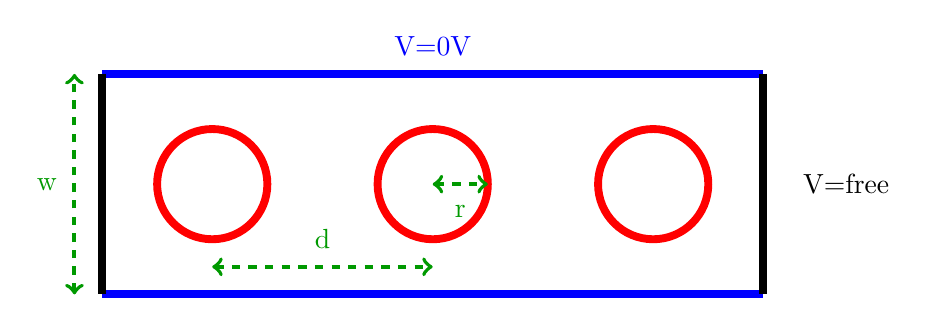
\begin{tikzpicture}[scale=0.7]
    \draw[line width=1mm, blue] (-6,3.5) -- (6,3.5);
    \draw[line width=1mm, blue] (-6,-0.5) -- (6,-0.5);
    \node at (0, 4) {\textcolor{blue}{V=0V}};

    \draw[line width=1mm, black] (-6,3.5) -- (-6,-0.5);
    \draw[line width=1mm, black] (6,3.5) -- (6,-0.5);
    \draw[line width=0.5mm, black!40!green, dashed, <->] (-6.5,-0.5) -- (-6.5,3.5);
    \node at (-7, 1.5) {\textcolor{black!40!green}{w}};
    \node at (7.5, 1.5) {\textcolor{black}{V=free}};

    \foreach \x in {-4,0,4} {
      \draw[line width=1mm,red] (\x,1.5) circle (1);
    }

    \draw[line width=0.5mm, black!40!green, <->, dashed] (0,1.5)--(1,1.5);
    \node at (0.5, 1) {\textcolor{black!40!green}{r}};

    \draw[line width=0.5mm, black!40!green, <->, dashed] (-4,0)--(0,0);
    \node at (-2, 0.5) {\textcolor{black!40!green}{d}};
	\end{tikzpicture}
\end{center}
\end{figure}

\begin{columns}
  \begin{column}{0.5\textwidth}

    \begin{itemize}
      \item number of strips
      \item strip radius \textcolor{black!40!green}{r}
      \item detector width \textcolor{black!40!green}{w}
    \end{itemize}

  \end{column}

  \begin{column}{0.6\textwidth}
    \begin{itemize}
      \item strip potential \textcolor{red}{V}
      \item inter strips centers distance \textcolor{black!40!green}{d}
    \end{itemize}

  \end{column}
\end{columns}

\end{frame}

\begin{frame}
  \frametitle{Pdetect software}
  \framesubtitle{Computing the potential: finite element method}

  \fontsize{12pt}{7.2}\selectfont


\textcolor{red}{Finite element method} solves $\nabla^2 V = 0$
numerically

\begin{itemize}
    \setlength\itemsep{1em}
  \item function domain is divided in \textcolor{red}{subdomains} called \textcolor{red}{finite elements}
  \item \textcolor{red}{piecewise interpolation}: one polynomial fits the restriction
  of the searched function on one finite element
  \item build a linear system with the polynomials coefficients
  \item solves the system thanks to constraints:
  \begin{itemize}
    \item satisfy $\nabla^2 V = 0$
    \item match imposed domain boundary conditions
    \item boundary conditions between polynomials defined on adjacent finite
    elements
    \end{itemize}
\end{itemize}

\end{frame}

\begin{frame}
  \frametitle{Pdetect software}
  \framesubtitle{Computing the potential: deal.ii}

\fontsize{13pt}{7.2}\selectfont

Use \textcolor{red}{deal.ii} to solve the Laplace eq. (fast thanks to multithreading)
\newline

\vspace{1.5em}

\begin{columns}
  \begin{column}{0.5\textwidth}

    \textcolor{red}{Inputs}:
      \begin{enumerate}
        \item Detector geometry
        \item Boundary conditions
        \item Max relative error on V
        %\item Maximum number of iterations
      \end{enumerate}

  \end{column}

  \begin{column}{0.6\textwidth}
    \textcolor{red}{Outputs} for each FE:
    \begin{enumerate}
      \item a funct approximating $V$
      \item a bound on the error on $V$
      \item a funct approximating $\nabla V$
    \end{enumerate}

  \end{column}
\end{columns}

\vspace{2em}

Perform this process \textcolor{red}{two times}
\begin{itemize}
  \item get $\textcolor{red}{\vec{E}} = -\nabla V$
  \item get $\textcolor{red}{\vec{E}_w} = -\nabla V_w$ with other boundary conditions
\end{itemize}
\end{frame}

\begin{frame}
  \frametitle{Pdetect software}
  \framesubtitle{Computing the potential: adaptive grid refinement (I)}

  \textcolor{red}{Electric field constant in most part of the detector}
  \begin{itemize}
    \item quick computation with large FE sufficient
  \end{itemize}

  But Electric field \textcolor{red}{varies strongly close to the strips}
  \begin{itemize}
    \item much smaller FE required to get precise results\newline
  \end{itemize}

  Uniform coarse grid composed of \textcolor{red}{large FE}

  $\implies$ results
  \textcolor{red}{not precise} enough close to the strips
  \newline

  Uniform dense grid composed of \textcolor{red}{small FE}

   $\implies$ \textcolor{red}{waste of time}

\end{frame}

\begin{frame}
  \frametitle{Pdetect software}
  \framesubtitle{Computing the potential: adaptive grid refinement (II)}

  Iterative process

  \begin{enumerate}
    \item Starts with the coarsest grid
    \item Compute $V$ and error at each FE
    \item If max error $>$ max tolerated error
    \begin{enumerate}
      \item \textcolor{red}{refine} only \textcolor{red}{cells} of the grid with \textcolor{red}{highest errors}
      \item return to step 2
    \end{enumerate}
  \end{enumerate}

  Final grid is composed of small cells only where the Electric field varies
  strongly
\end{frame}

\begin{frame}
  \frametitle{Pdetect software}
  \framesubtitle{Serrated rectangle: potential and electric field}

  \fontsize{10pt}{7.2}\selectfont


  Strip potential = 200V, detector width = 300$\mu$m, strip length = 100$\mu$m, strip width = 20$\mu$m,
  inter-strips distance = 100$\mu$m, max relative error = 0.9$\%$

  \vspace{-2em}

  \begin{center}
  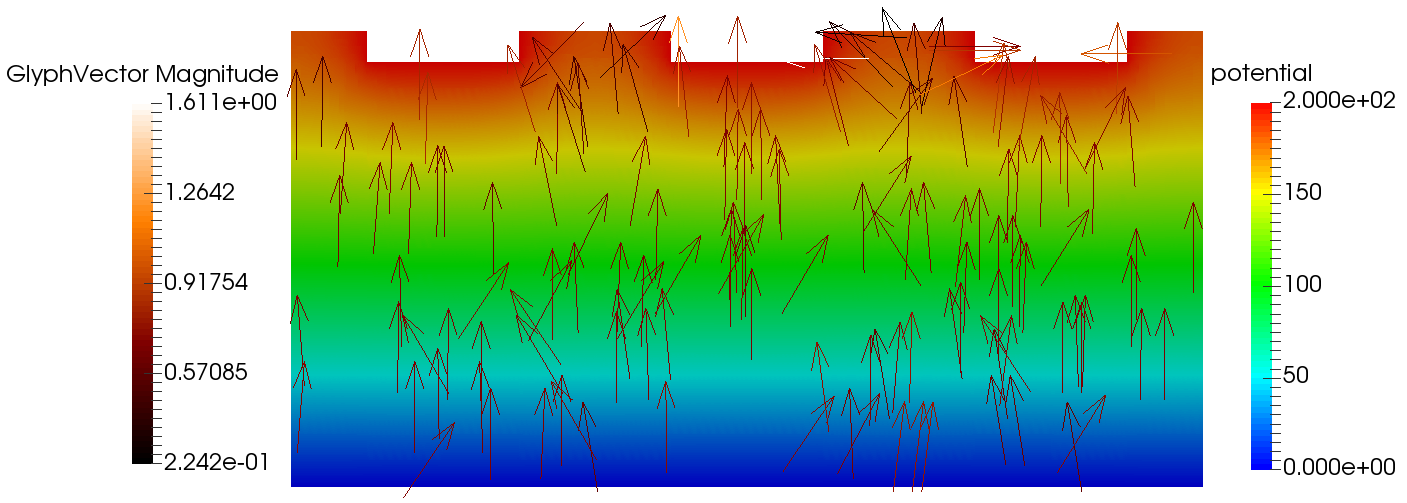
\includegraphics[scale=0.18]{images/serrated_pot_3.png}
  \end{center}

\vspace{-2em}

  \begin{center}
  \hspace{4.5em} 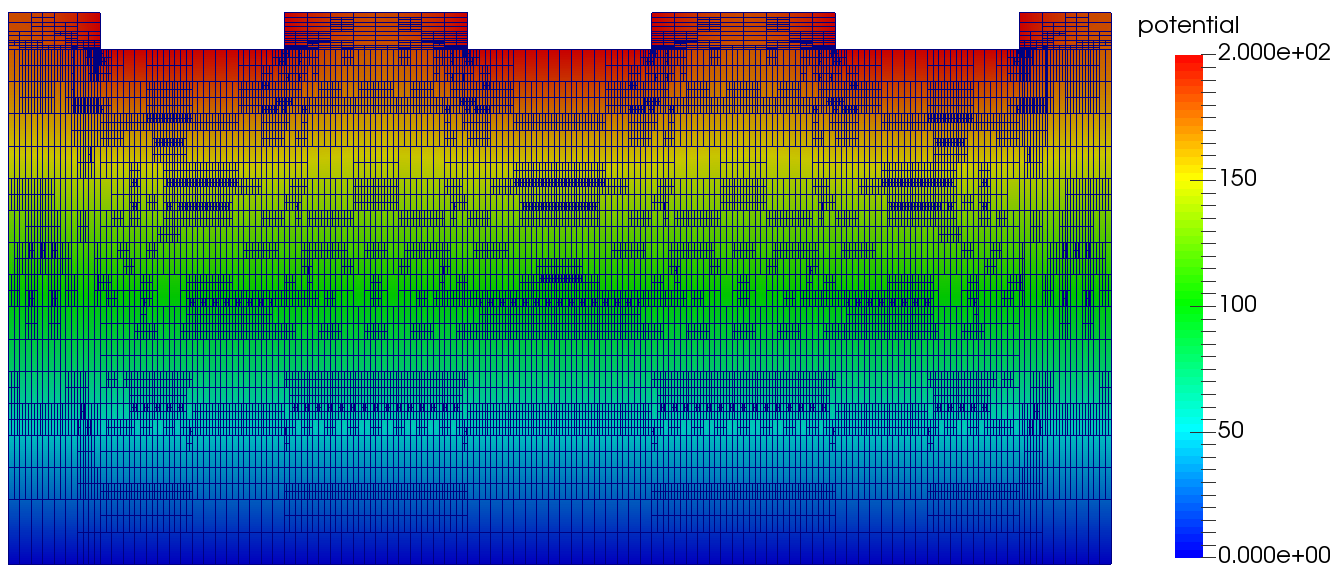
\includegraphics[scale=0.15]{images/serrated_pot_3_grid.png}
  \end{center}

\end{frame}

\begin{frame}
  \frametitle{Pdetect software}
  \framesubtitle{Serrated rectangle: weighting potential and weighting electric field}

  \fontsize{10pt}{7.2}\selectfont


  Strip potential = 200V, detector width = 300$\mu$m, strip length = 100$\mu$m, strip width = 20$\mu$m,
  inter-strips distance = 100$\mu$m, max relative error = 0.9$\%$

  \vspace{-2em}

  \begin{center}
  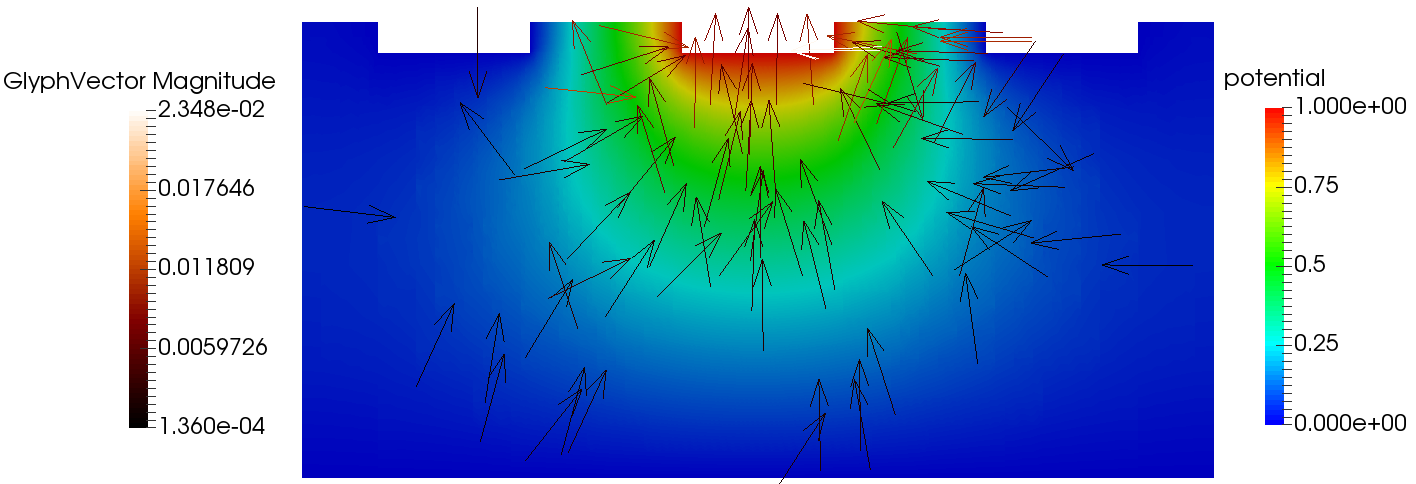
\includegraphics[scale=0.175]{images/serrated_pot_3_weight.png}
  \end{center}

\vspace{-2em}

  \begin{center}
  \hspace{4em} 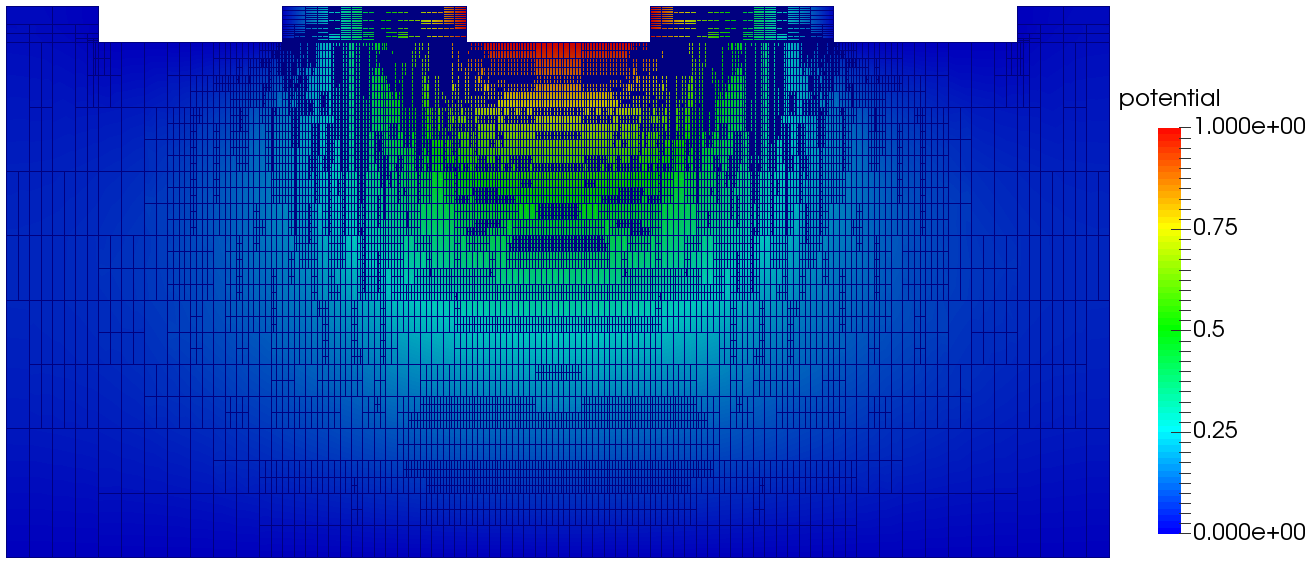
\includegraphics[scale=0.15]{images/serrated_pot_3_grid_weight.png}
  \end{center}

\end{frame}

\begin{frame}
  \frametitle{Pdetect software}
  \framesubtitle{Rectangular strips: potential and electric field}

  \fontsize{10pt}{7.2}\selectfont


  Detector width = 200 $\mu$m, strip length = 50 $\mu$m, strip width = 50 $\mu$m,
	inter strips distance = 100$\mu$m, number of strips = 3, potential = 10V,
	max relative error = 0.9$\%$

  \begin{center}
  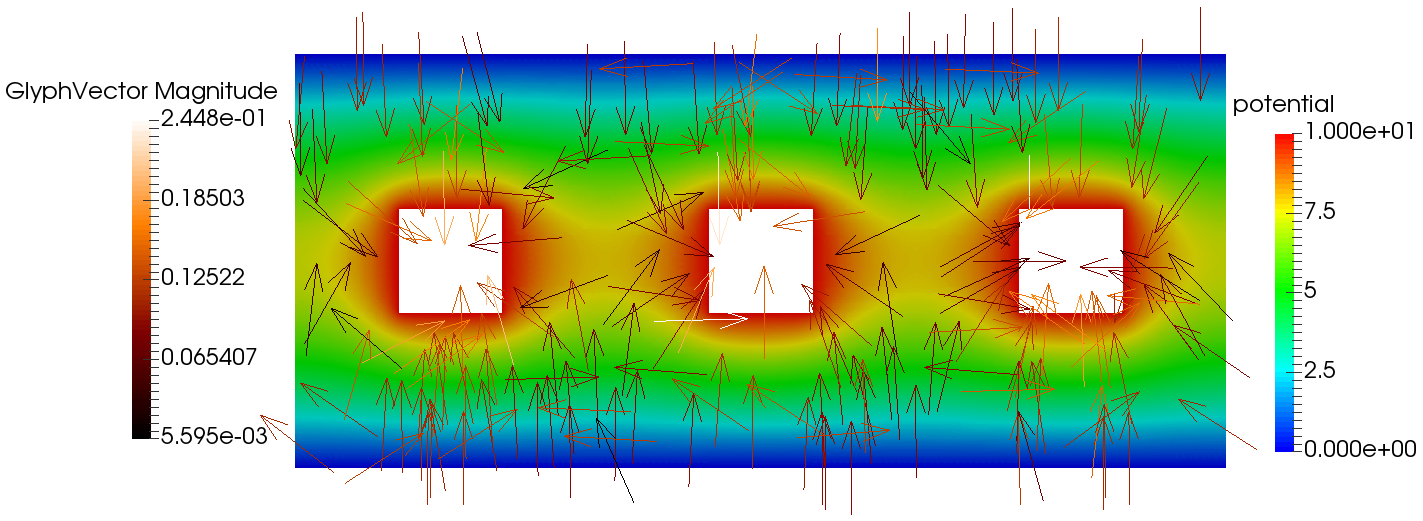
\includegraphics[scale=0.175]{images/rect_rect_pot_3.png}
  \end{center}

\vspace{-2em}

  \begin{center}
  \hspace{4em} 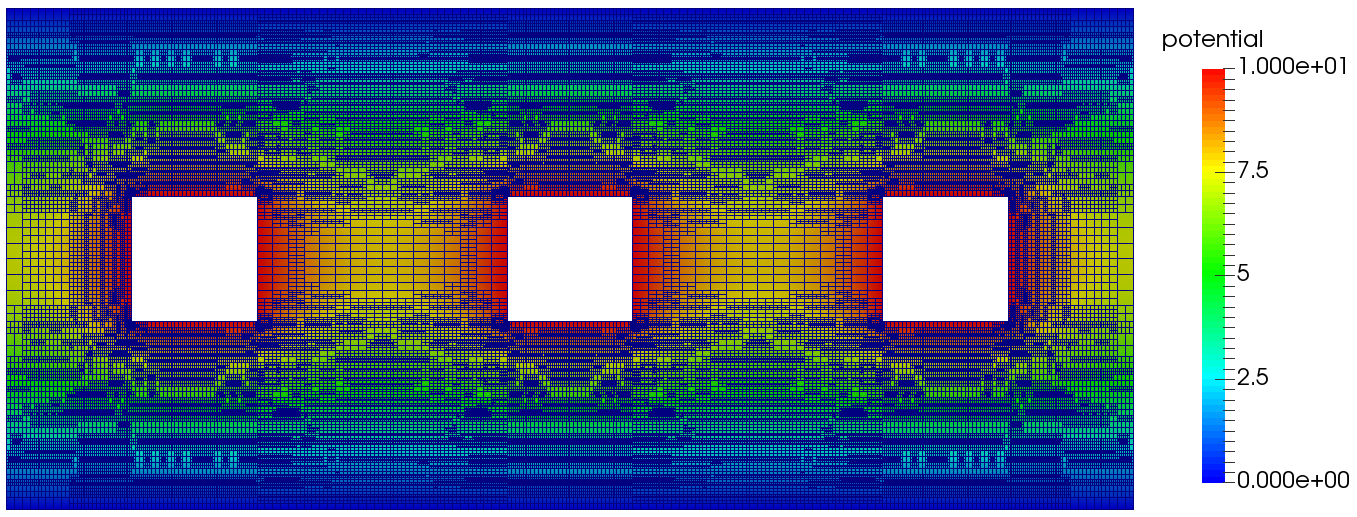
\includegraphics[scale=0.15]{images/rect_rect_pot_3_grid.png}
  \end{center}

\end{frame}

\begin{frame}
  \frametitle{Pdetect software}
  \framesubtitle{Rectangular strips: weighting potential and weighting electric field}

  \fontsize{10pt}{7.2}\selectfont


  Detector width = 200 $\mu$m, strip length = 50 $\mu$m, strip width = 50 $\mu$m,
	inter strips distance = 100$\mu$m, number of strips = 3, potential = 10V,
	max relative error = 0.9$\%$

  \begin{center}
  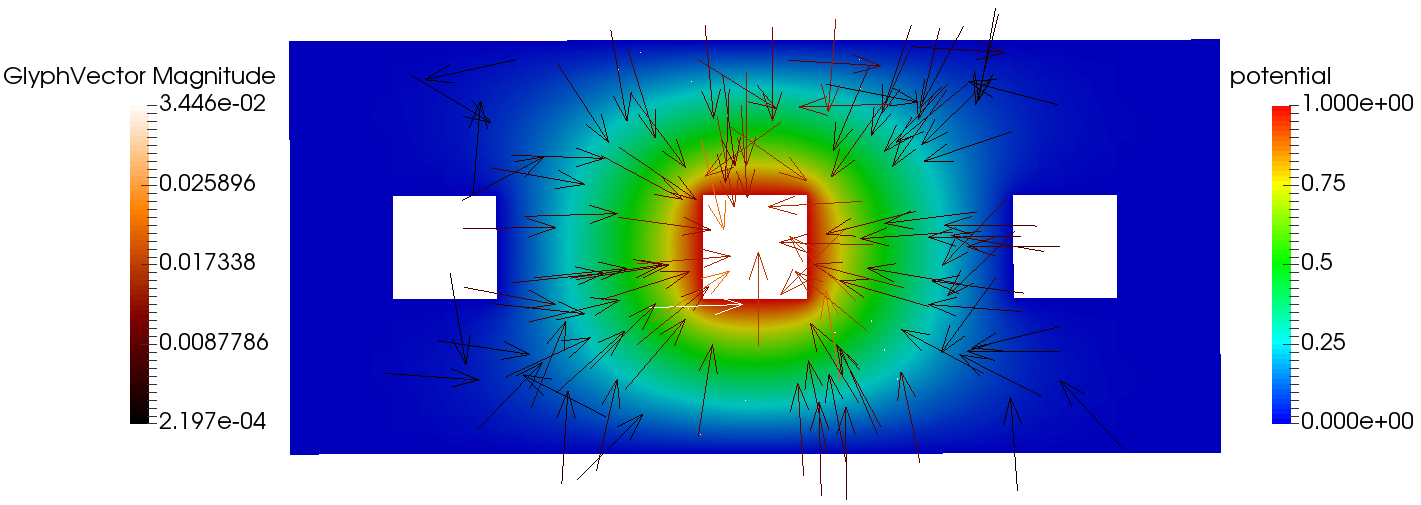
\includegraphics[scale=0.18]{images/rect_rect_pot_3_weight.png}
  \end{center}

\vspace{-2em}

  \begin{center}
  \hspace{4em} 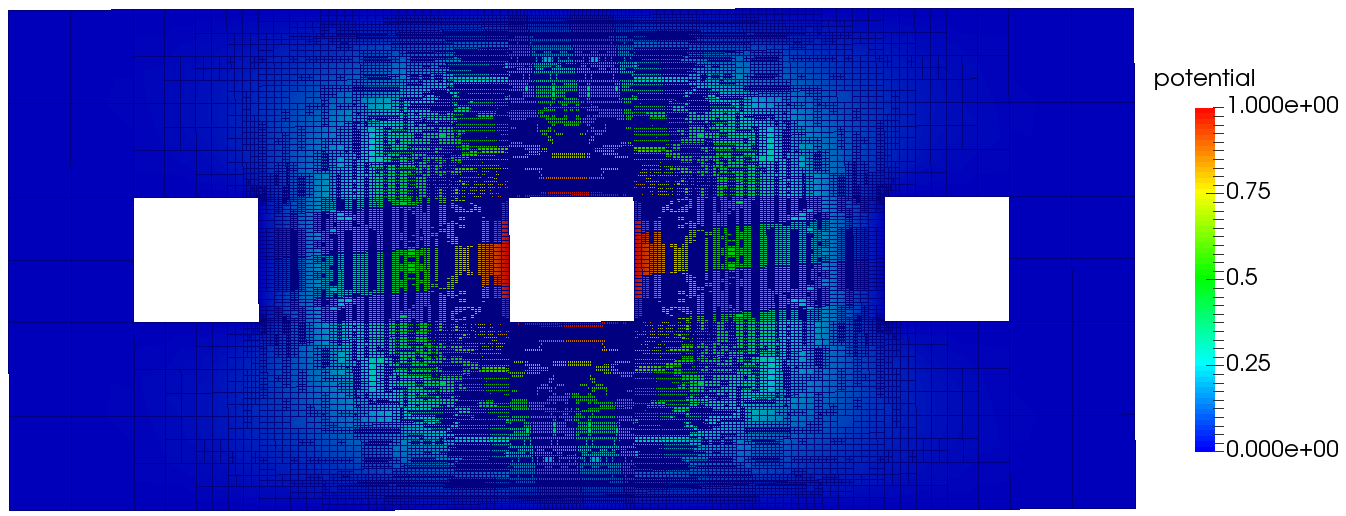
\includegraphics[scale=0.15]{images/rect_rect_pot_3_weight_grid.png}
  \end{center}

\end{frame}

\begin{frame}
  \frametitle{Pdetect software}
  \framesubtitle{Circular strips: potential and weighting potential}

  \fontsize{10pt}{7.2}\selectfont

Detector width = 200$\mu$m, number of strips = 3, radius = 21$\mu$m,
 inter strips distance = 50$\mu$m, potential = 10V, max relative error 1$\%$

 \begin{columns}
   \begin{column}{0.5\textwidth}

     \begin{center}
     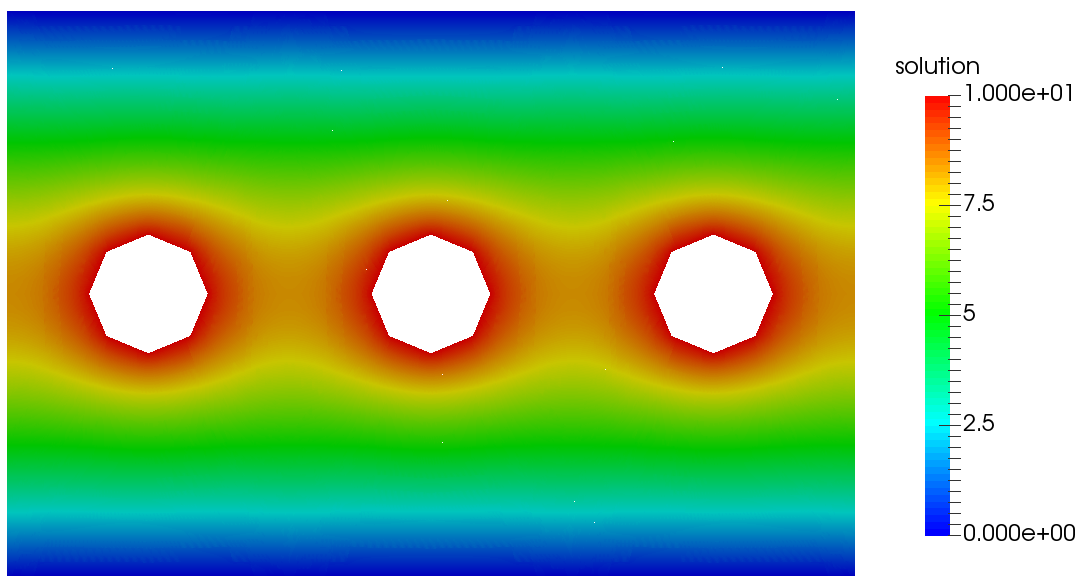
\includegraphics[scale=0.16]{images/circle_pot_3.png}
     \end{center}

   \end{column}

   \begin{column}{0.5\textwidth}
     \begin{center}
       \vspace{0.5em}
     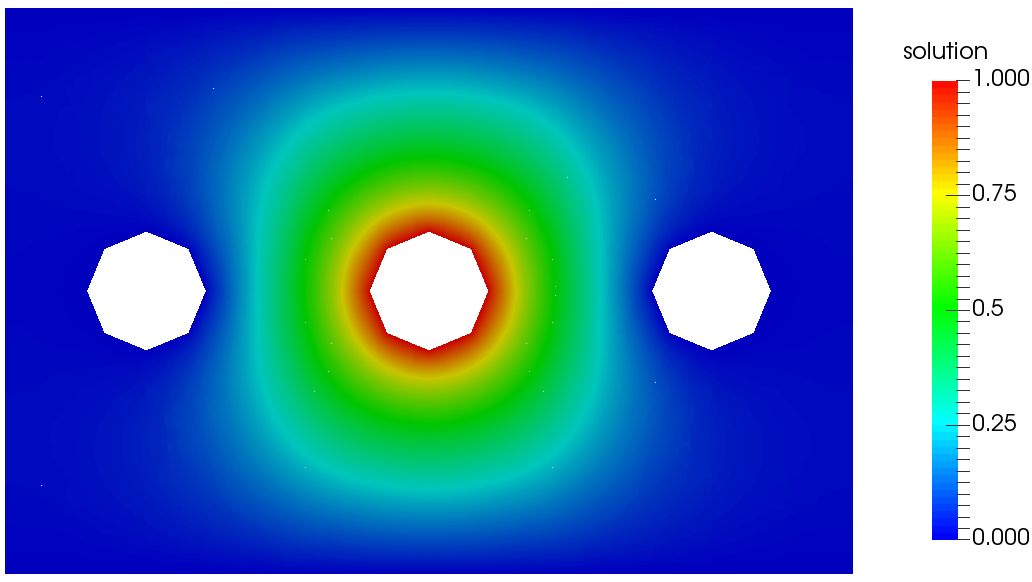
\includegraphics[scale=0.16]{images/circle_pot_3_weight.png}
     \end{center}

   \end{column}
 \end{columns}

\end{frame}

{
\usebackgroundtemplate{
\includegraphics[width=\paperwidth, height=\paperheight]{images/circle_pot_3_weight_grid.png}}
\begin{frame}
  \frametitle{Pdetect software}
  \framesubtitle{Circular strips: example of adaptive grid}

  % \begin{center}
  %    
\includegraphics[scale=0.18]{images/circle_pot_3_weight_grid.png}
  %  \end{center}

\end{frame}
}
%
% \begin{frame}
%   \frametitle{Pdetect software}
%   \framesubtitle{Potential numerical vs analytical solution}
%
%   \begin{columns}
%     \begin{column}{0.5\textwidth}
%
%       \begin{center}
%         \textcolor{red}{Analytical}
%         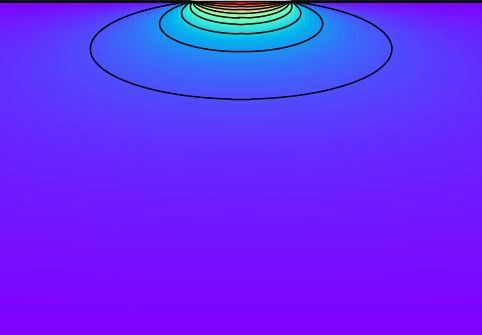
\includegraphics[width=\textwidth]{images/plot_analytic.png}
%       \end{center}
%
%     \end{column}
%
%     \begin{column}{0.5\textwidth}
%       \begin{center}
%         \textcolor{red}{Numerical}
%       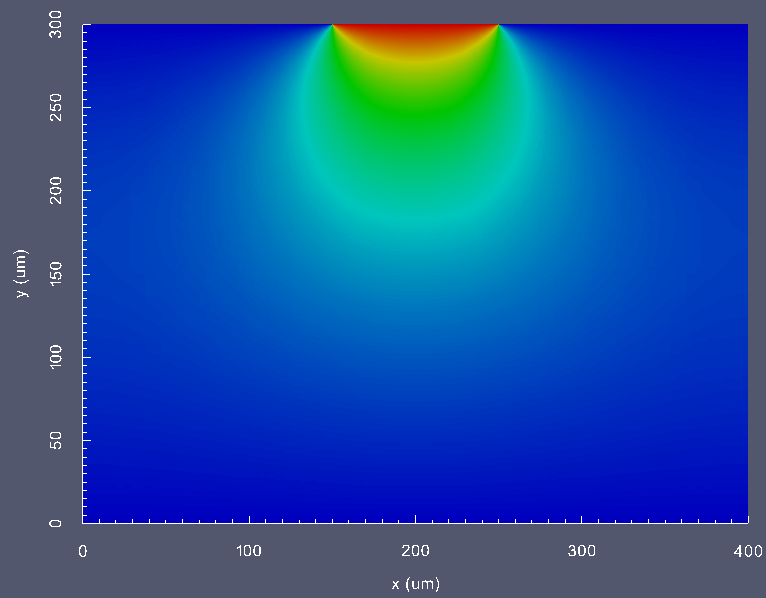
\includegraphics[width=\textwidth]{images/w_semi_free_conditions.png}
%       \end{center}
%
%     \end{column}
%   \end{columns}
%
% \end{frame}

\begin{frame}
  \frametitle{Pdetect software}
  \framesubtitle{Potential: numerical vs analytical solution}

  \fontsize{10pt}{7.2}\selectfont

  Potential along a vertical line (middle of the detector)

  Pitch = 400$\mu$m, strip length = 100$\mu$m, width = 300$\mu$m, V$_{strip} = 1$V

\vspace{-2em}

  \begin{columns}
      \begin{column}{0.5\textwidth}

        \begin{center}
          \begin{tikzpicture}
            \node[inner sep=0pt]  at (0,0) {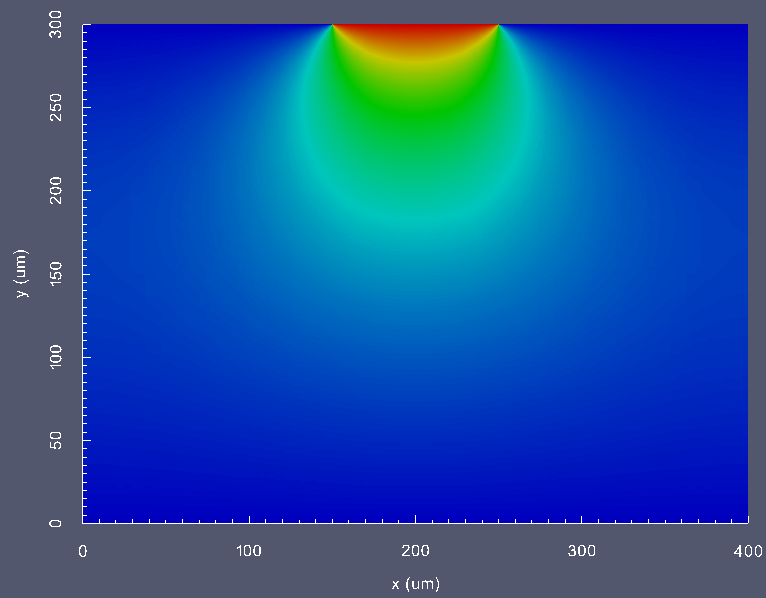
\includegraphics[width=\textwidth]{images/w_semi_free_conditions.png}};
            \draw[red, line width=0.5mm, dashed] (0.23,-1.6) -- (0.23,1.95);
          \end{tikzpicture}
        \end{center}
      \end{column}

      \begin{column}{0.5\textwidth}
        \begin{center}
          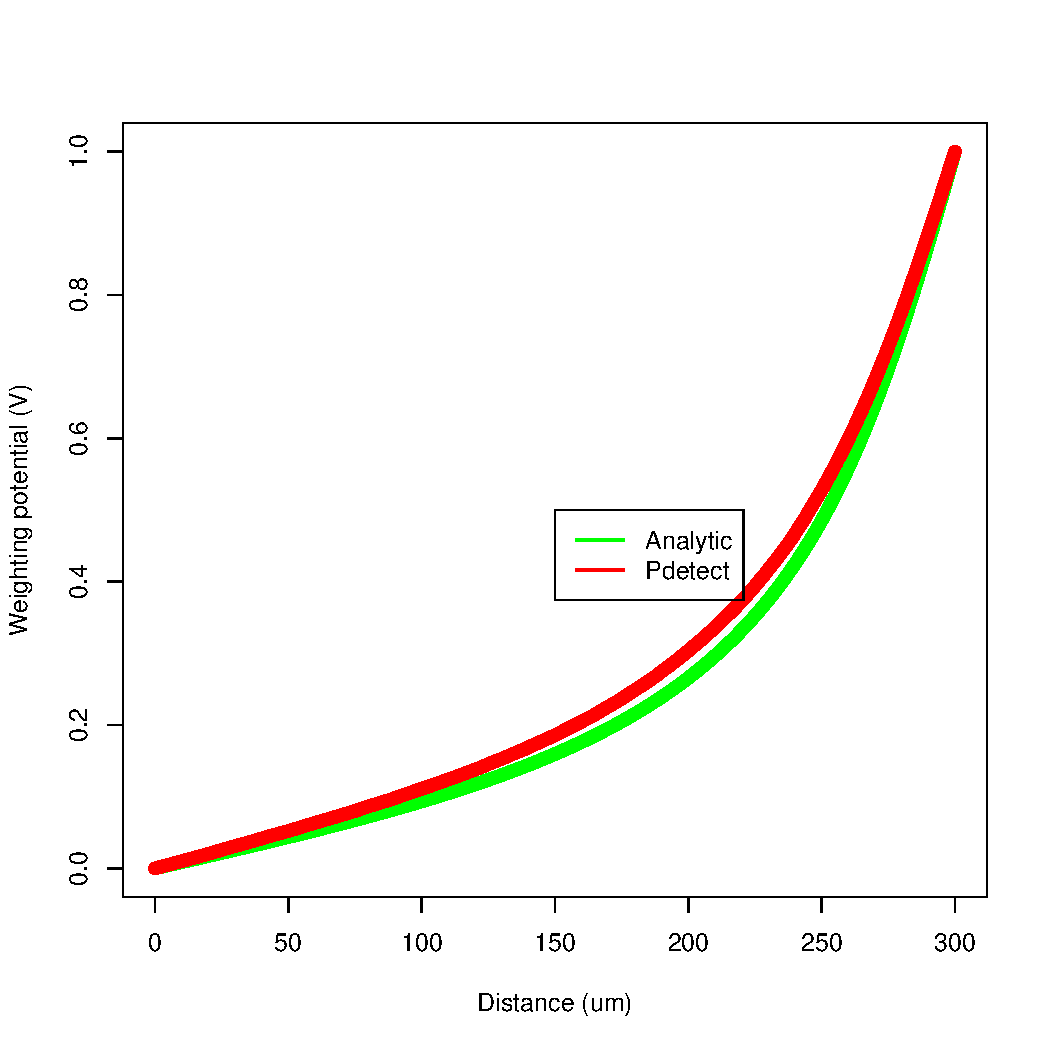
\includegraphics[width=\textwidth]{images/semi-free.pdf}
        \end{center}

      \end{column}
    \end{columns}

\begin{itemize}
  \item The two curves perfectly match for a different strip width
  \item Strip width used to compute analytical solution is unknown
\end{itemize}

\end{frame}

\begin{frame}
  \frametitle{Pdetect software}
  \framesubtitle{Potential: comparison with Weightfield}

  \fontsize{10pt}{7.2}\selectfont

  V=1V, 1 strip, pitch = 450$\mu$m, strip length = 100$\mu$m, width = 300$\mu$m

  \begin{columns}

      \begin{column}{0.1\textwidth}
        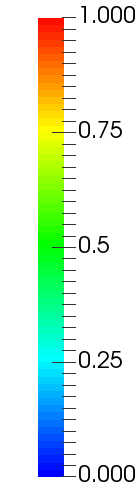
\includegraphics[width=\textwidth]{images/legend_weight_pot.png}
      \end{column}

      \begin{column}{0.43\textwidth}

        \begin{center}
          %\begin{tikzpicture}
            %\node[inner sep=0pt]  at (0,0) {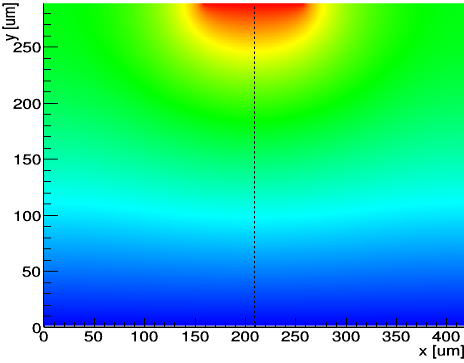
\includegraphics[width=\textwidth, height=6cm]{images/weight_free.png}};
          %\end{tikzpicture}
          \textcolor{red}{Weightfield}
          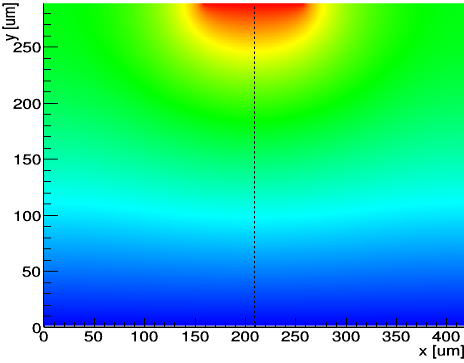
\includegraphics[width=\textwidth]{images/weight_free.png}
        \end{center}
      \end{column}

      \begin{column}{0.47\textwidth}
        \begin{center}
          %\vspace{1.28em}
          \vspace{0.5em}

          \textcolor{red}{Pdetect}

            \vspace{0.3em}

          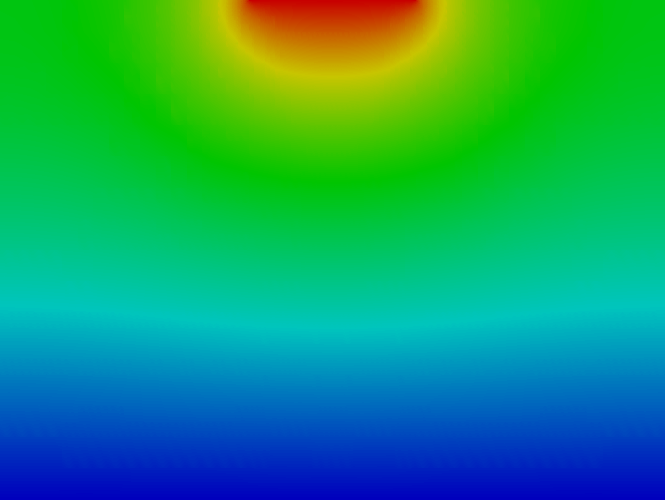
\includegraphics[width=\textwidth]{images/w_free_conditions.png}
        \end{center}

      \end{column}
    \end{columns}

\end{frame}


\begin{frame}
  \frametitle{Appendix}
  \framesubtitle{Media ionization}

  Number of \textcolor{red}{hole-electron pairs}

  \[N = \frac{dE/dx}{w} \times L\]

\begin{itemize}
  \item \textcolor{red}{$dE/dx$} energy deposited per unit of length
  \item \textcolor{red}{$w$} energy to produce one hole-electron pair
  \item \textcolor{red}{$L$} distance covered in the detector
\end{itemize}

\end{frame}

\begin{frame}
  \frametitle{Appendix}
  \framesubtitle{Saturation}

  \begin{equation}
		\mu_s = \mu \left (1 + \left (\frac{\mu |E_y|}{v_{sat}} \right )^{\beta} \right )^{-\frac{1}{\beta}}
		\label{eq:saturation}
	\end{equation}

\begin{itemize}
  \item $\beta$ is a constant
  \item $\mu$ is the mobility when not considering saturation
  \item $E_y$ is the component of the electric field along the axis orthogonal
  to the anode and cathode
  \item $v_{sat}$ the saturation velocity, it depends on the media and the
  temperature.
\end{itemize}

\end{frame}

\begin{frame}
  \frametitle{Appendix}
  \framesubtitle{Townsend avalanche}

  During $\Delta t$ the initial electric charge $q_0$ is multiplied:

  \begin{equation}
    q = q_0 e^{\alpha \Delta x}
    \label{eq:townsend}
  \end{equation}

\begin{itemize}
  \item $\Delta x$: distance covered by the e$^-$ during $\Delta t$
  \item $\alpha$ is the \textcolor{red}{first Townsend coefficient}

  \[\alpha = ap \ e^{-bp/E}\]

  $a, b$: constants depending on the gas media

  $p$: pressure in the detector

  $E$: norm of the electric field at the charge position
\end{itemize}

\end{frame}

\begin{frame}
  \frametitle{Appendix}
  \framesubtitle{Model-view-controller}


\fontsize{12pt}{7.2}\selectfont

  \begin{columns}
    \begin{column}{0.4\textwidth}

      \begin{itemize}
        \item \textcolor{red}{model} manages the data, logic and rules of the application
        \item \textcolor{red}{view}: any output representation of information, multiple views of the same information are possible
        \item \textcolor{red}{controller} accepts input and converts it to commands for the model or view
      \end{itemize}

    \end{column}

    \begin{column}{0.5\textwidth}
      \begin{center}
        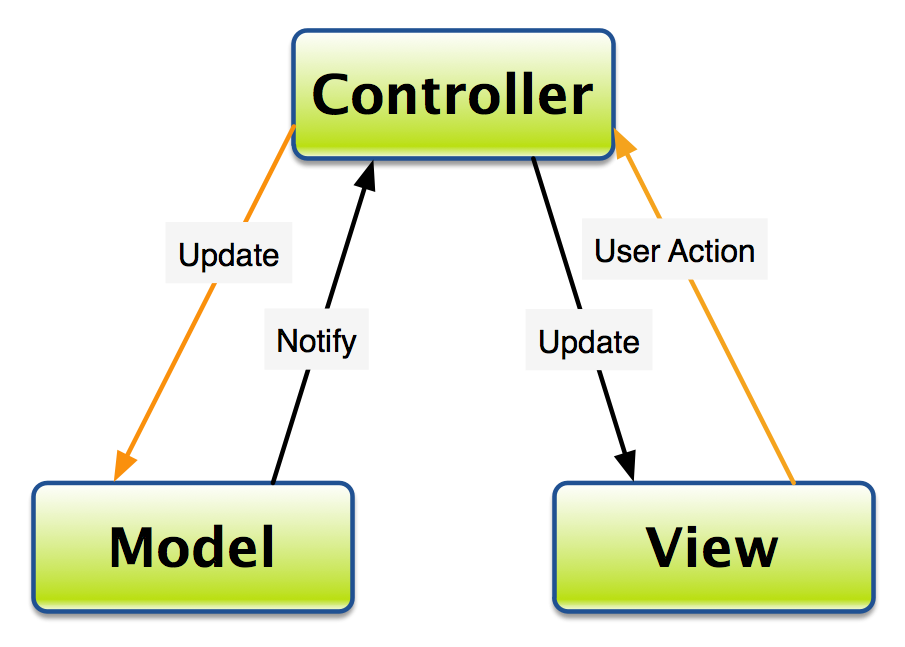
\includegraphics[scale=0.45]{images/MVC.png}
      \end{center}

    \end{column}
  \end{columns}

\end{frame}

\begin{frame}
  \frametitle{Appendix}
  \framesubtitle{Potential analytical solution}

\begin{center}
  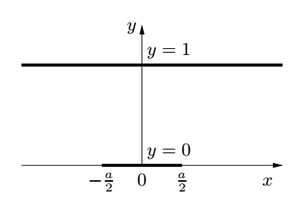
\includegraphics[scale=0.5]{images/analytic.png}
\end{center}

\vspace{-1.5em}

  \[\phi_w(x,y) = atan\left({\sin(\pi y)\sinh(\pi {a\over{2}})\over
      {\cosh(\pi x)-\cos(\pi y)\cosh(\pi {a\over{2}})}}\right)\]

\end{frame}

\begin{frame}
  \frametitle{Appendix}
  \framesubtitle{Potential: numerical vs analytical solution (I)}

  \fontsize{10pt}{7.2}\selectfont

  Potential along a vertical line (edge of the strip)

  Pitch = 400$\mu$m, strip length = 100$\mu$m, width = 300$\mu$m, V$_{strip} = 1$V

\vspace{-1.5em}

  \begin{columns}
      \begin{column}{0.5\textwidth}

        \begin{center}
          \begin{tikzpicture}
            \node[inner sep=0pt]  at (0,0) {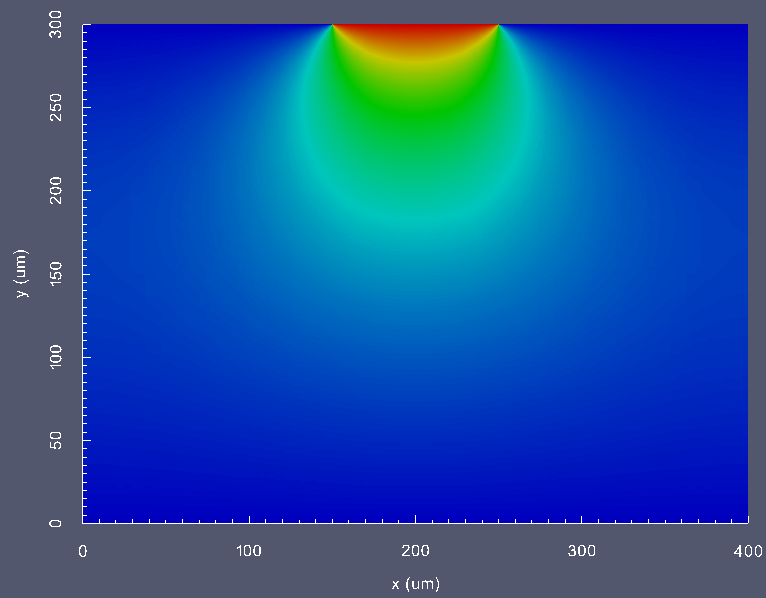
\includegraphics[width=\textwidth]{images/w_semi_free_conditions.png}};
            \draw[red, line width=0.5mm, dashed] (-0.35,-1.6) -- (-0.35,1.95);
          \end{tikzpicture}
        \end{center}
      \end{column}

      \begin{column}{0.5\textwidth}
        \begin{center}
          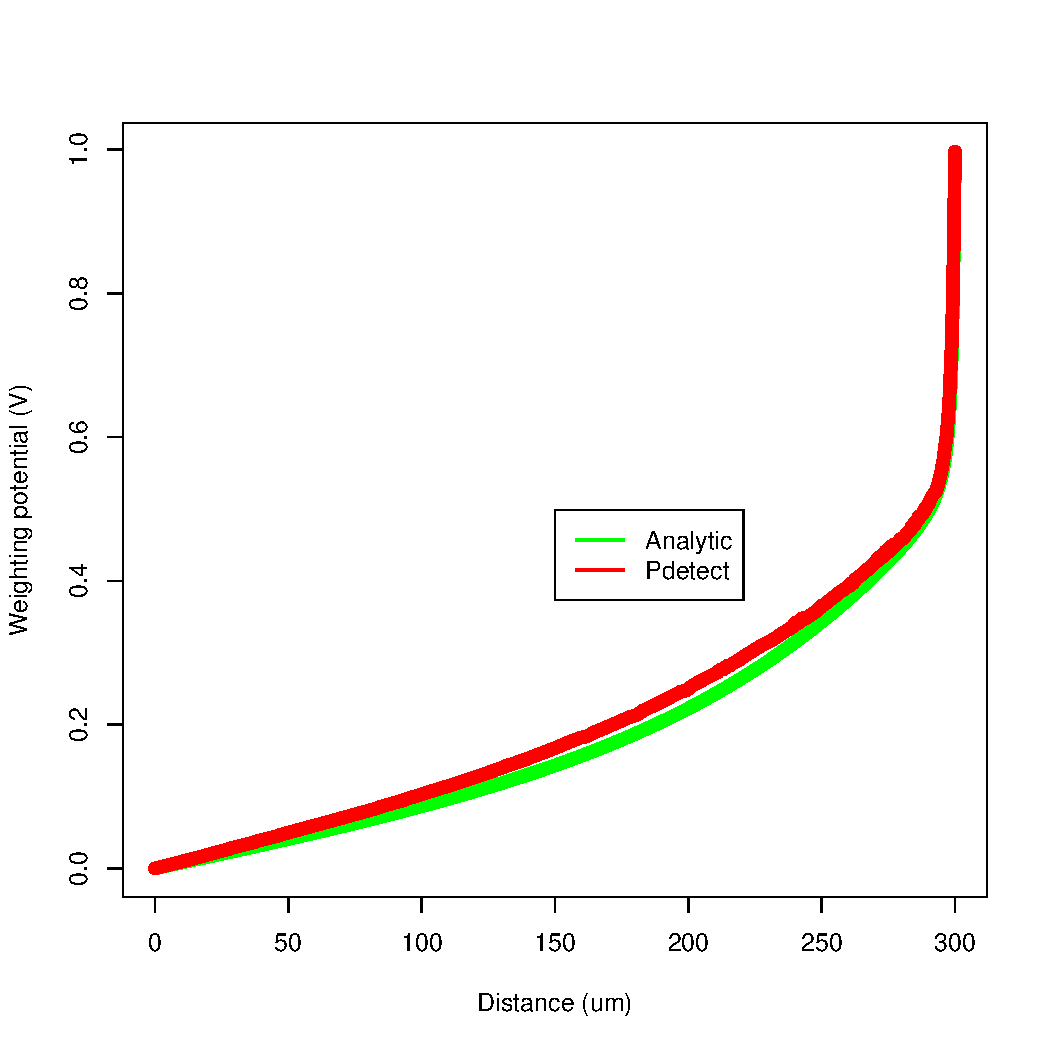
\includegraphics[width=\textwidth]{images/edge-strip.pdf}
        \end{center}

      \end{column}
    \end{columns}

\end{frame}

\begin{frame}
  \frametitle{Appendix}
  \framesubtitle{Potential: numerical vs analytical solution (II)}

  \fontsize{10pt}{7.2}\selectfont

  Potential along a horizontal line (below the strip at y=298 $\mu$m)

  Pitch = 400$\mu$m, strip length = 100$\mu$m, width = 300$\mu$m, V$_{strip} = 1$V

\vspace{-1.5em}

  \begin{columns}
      \begin{column}{0.5\textwidth}

        \begin{center}
          \begin{tikzpicture}
            \node[inner sep=0pt]  at (0,0) {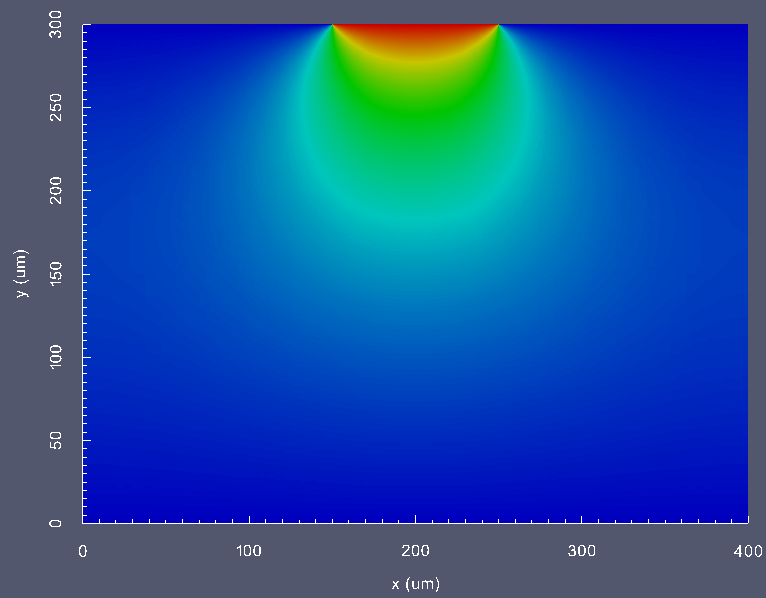
\includegraphics[width=\textwidth]{images/w_semi_free_conditions.png}};
            \draw[red, line width=0.5mm, dashed] (-2.1,1.9) -- (2.6,1.9);
          \end{tikzpicture}
        \end{center}
      \end{column}

      \begin{column}{0.5\textwidth}
        \begin{center}
          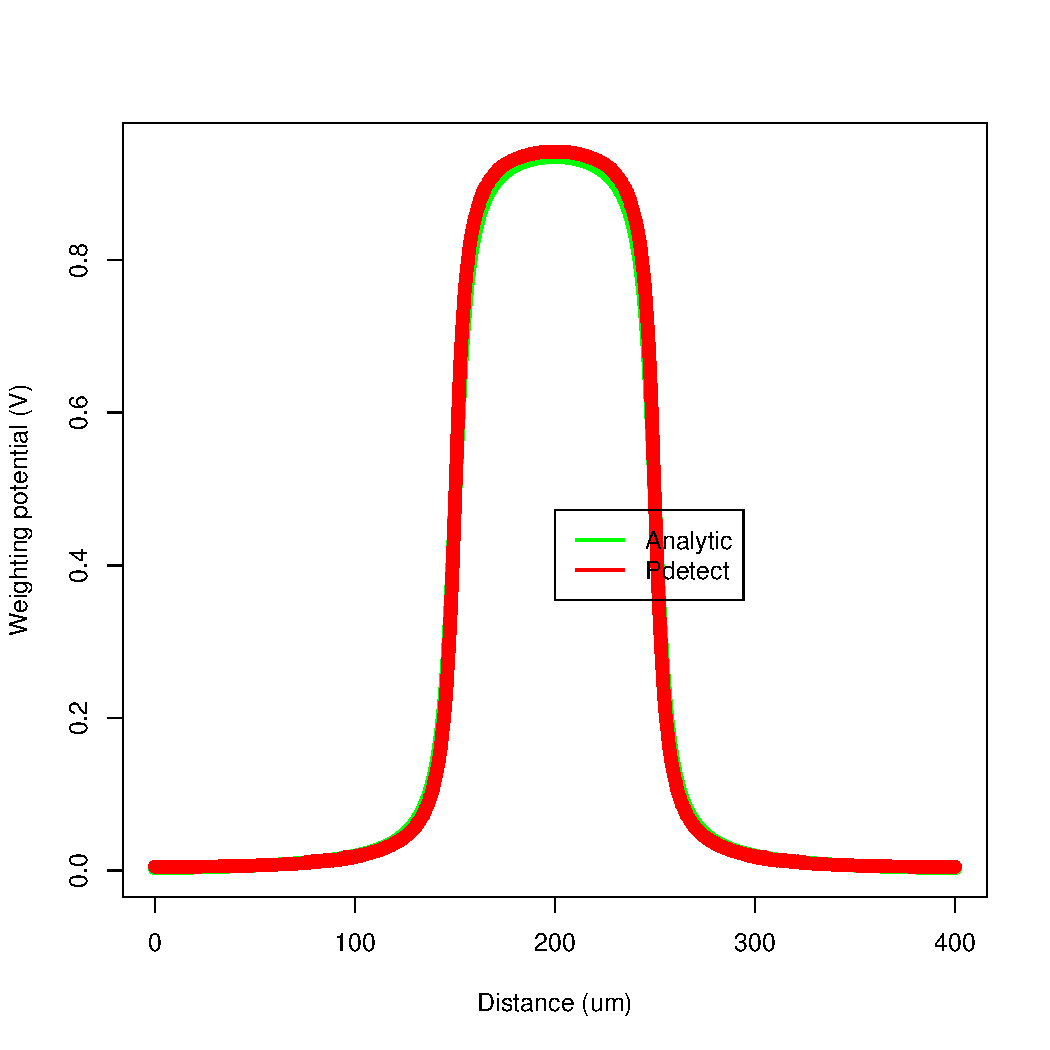
\includegraphics[width=\textwidth]{images/horizon-top.pdf}
        \end{center}

      \end{column}
    \end{columns}

\end{frame}

\end{document}
